\section{Theoretical Analysis}
\label{sec:analysis}

\par In this section, we will analyse our theoretical model of the AC/DC converter in terms of the DC output voltage $V_O$ and the deviation from this DC value, the AC component $v_o$. Our goal is to maximize the merit function given by:

\begin{equation}
M=\frac{1}{cost*(ripple(v_O)+average(v_O-12)+10^{-6}}
  \label{eq:merit}
\end{equation}
With cost given by:
\begin{equation}
M=\frac{\text{Sum of the resistors}}{1000}+\frac{Capacity}{10^{-6}}+Num_{diodes}*0.1
  \label{eq:cost}
\end{equation}
 
\par To maximize it we should obtain small deviations from $V_O$ (small riplle) and obtain a $V_O$ closer to $12V$, wich is the output voltage required. At the same time, we must reduce the cost of the circuit, by reducing the number of components and their values. We concluded that the following values were the ones that maximize this function: $C=920\mu F$, $R_e=920k\Omega$ , $R_v=3.3k\Omega$.
 
\subsection{Transformer and full wave bridge rectifier}
\label{subsec:full_wave_rectifier}

\par For the first part of the circuit we used a transformer that converts the input voltage $v_S=230cos(\omega t) V$, with $\omega=2\pi*50$, to a voltage with the same frequency and a amplitude of $230.1V$. Thus, the number of spirals for the transformer was $N=\frac{N_1}{N_2}=1.000434783$.

\par After that, we introduced a full wave rectifier circuit that converts the negative values to positive ones, so the peaks of the sinusoidal voltage appear with the double of the original frequency. Thus, the voltage that enters the envelope detector is $v_3=|230.1cos(\omega*t)|$. To do that, we use a circuit with 4 diodes (between nodes 0, 1, 2 and 3) which ensures that the output voltage is always positive, because they only conduct current in the forward active region.
\par In that way, one can reduce the ripple in the envelope detector circuit, as we will se in the next chapter.

\subsection{Envelope Detector}
\label{subsec:env}

\par The main purpose of the envelope detector is to obtain a voltage that follows the peaks of the input voltage, achieving much smaller AC components. We can distinguish 2 phases of operation, considering the ideal diode model:

\begin{itemize}
  \item When the diode is on, the envelope voltage $v_4$ is equal to $v_3$. This happens for $T_{ON}<t<T_{OFF}$, every period. 
  \item When the diode is off, it blocks the current, and the voltage in the capacitor starts discharging throuth the resistor $R_e$. The equation to compute the voltage when the diode is off is:
\begin{equation}
  v_4=230.1*(2\omega T_{OFF})*\exp{(-\frac{t-T_{OFF}}{R_eC})}
\end{equation}
\end{itemize}

 \par For computing $T_{OFF}$ we used the equation
 
  \begin{equation}
T_{OFF}=\frac{1}{2\omega}*\arctan(\frac{1}{2\omega*R_e*C})
  \label{eq:toff}
  \end{equation}
\par Then we can solve the implicit equation for $T_{ON}$:

\begin{equation}
v_3(T_{ON})=230.1\cos(2*\omega*T_{OFF})\exp{(-\frac{T_{ON}-T_{OFF}}{R_e*C})}
  \label{eq:ton}
\end{equation}

\par Notice that the envelope output voltage is defined by branches. We computed the DC value of $v_4$ as $V_4=mean(v_4)$, and the ripple is the maximum deviation $ripple_envelope=max(v_4)-min(v_4)$. This ripple is reduced by doubling the frequency in the full wave bridge rectifier, because the difference between $T_{ON}$ and $T_{OFF}$ is shorter. In this table we present the values for the DC component and the ripple:

\begin{table}[H]
    \centering
    \begin{tabular}{|l|r|}
    \hline    
    {\bf Name} & {\bf Value (V)} \\ \hline
    $Ripple_{envelope}$ & $0.002240$ \\ \hline 
$Average_{envelope}$ & $22.498882$ \\ \hline 

    \end{tabular}
     \caption{Output DC voltage and ripple for the envelope detector.}
    \label{tab:env}
  \end{table}


The next plot shows the rectified voltage, $v_3$, and the envelope output voltage covering the peaks, $v_4$. 

\begin{figure}[H] \centering
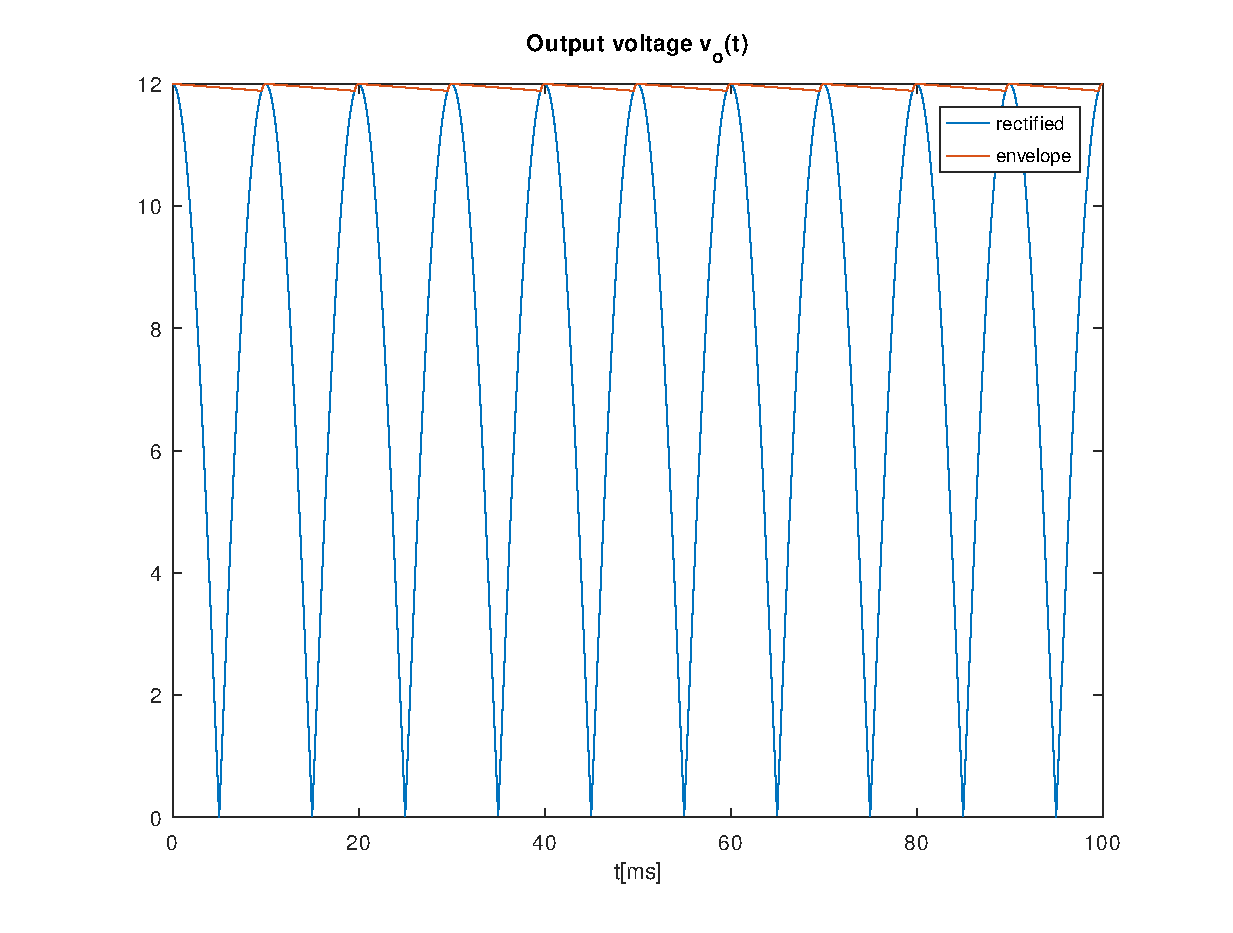
\includegraphics[width=0.8 \linewidth]{venvlope.eps}
\caption{Rectified and envelope voltages in function of time.}
\label{fig:env}
\end{figure}

\subsection{Voltage regulator}
\label{subsec:reg}

\par The next stage is the voltage regulator, composed by 17 diodes and a resistor $R_v$. The diodes impose a DC output voltage, $V_O$, close to 12V, that was our goal to maximize the merit equation \ref{eq:cost}. By using a large resistor, we apply a voltage division in incremental terms. Therefore, one can reduce the AC component of the output voltage, $v_4$, and his ripple. We did an operating point and incremental analysis on this part of the circuit, assuming that the AC component of $v_4$ is already small.

\par To compute the operating point, we circulate the mesh composed by the diodes and the resistor $R_v$ and obtained the following equation (using only the DC component of the voltages):

\begin{equation}
 -V_4+IS*Id*R2+V_O=0
  \label{eq:reg_mesh}
\end{equation}
 
 \par Where $Id$ is the DC component of the current that passe throuth the diodes, giver by:
 
\begin{equation}
I_d=I_S*\exp{(\frac{V_O}{17*\eta*V_T})}
\label{eq:Id}
\end{equation}
 
 \par $I_S$, $\eta$ and $V_T$ are constants for the diode model used. Solving this implicit equation with Newton-Raphson methods one can obtain the DC output $V_O$, which we want to be close to 12V.  
 \par Then we compute $V_{ON}$, which is the threshold voltage to achieve the active region of an ideal diode model, that can be estimated as $V_{ON}=\frac{V_O}{17}$. Using this method instead of chosing a fixed $V_{ON}$, one can reproduce with less error the DC output given by the simulation.
 
 \par For the incremental analysis, we computed the incremental resistor of the 17 diodes:
 
\begin{figure}[H] \centering
\includegraphics[width=0.5 \linewidth]{volt_regulator.pdf}
\caption{Circuit model used for incremental analysis.}
\label{fig:env}
\end{figure}
 
\begin{equation}
r_d=\frac{\eta*V_T}{I_S*\exp{(\frac{V_{ON}}{\eta*V_T})}}
\label{eq:rd}
\end{equation}

\par Then we applied a voltage divisor to compute the AC component $v_o$ for every time step of the $v_O$ output voltage:

 \begin{equation}
 v_O(t)=\frac{17*rd}{17*rd+R_v}*(v_4(t)-V_4)
  \label{eq:reg}
\end{equation}

\par Those are the $ripple=max(v_O)-min(v_O)$ and the DC output, $V_O$, obtained with the same input values values we used in the simulation:

\begin{table}[htb!]
  \centering
  \begin{tabular}{|l|r|}
      \hline    
      {\bf Name} & {\bf Value [V]} \\ \hline
      $Ripple_{regulator}$ & $0.000076$ \\ \hline 
$Average_{regulator}$ & $11.822949$ \\ \hline 

  \end{tabular}
\quad
  \begin{tabular}{|l|r|}
    \hline    
    {\bf Name} & {\bf Value [V]} \\ \hline
    Merit & $0.005627$ \\ \hline 

  \end{tabular}
     \caption{Output DC voltage and ripple for the voltage regulator. Merit obtained with theoretical analysis.}
  \label{tab:reg}
\end{table}


\par As we will see in the next chapter, this value of merit is much smaller than the one obtained with the simulation in ngspice, in part because of simplifications in the models used.

\par Next we show some plots of the voltages obtained:

 \begin{figure}[H] \centering
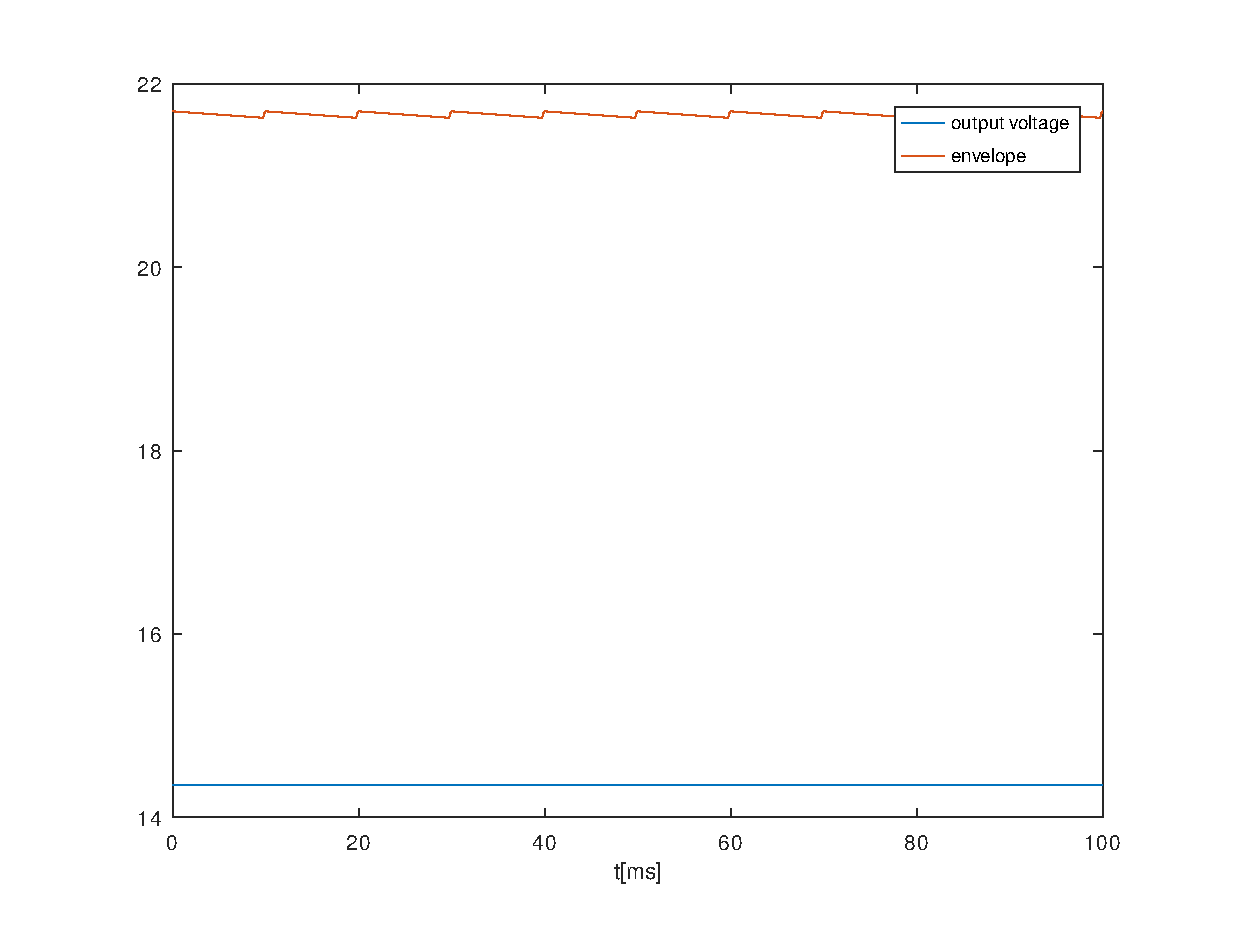
\includegraphics[width=0.8 \linewidth]{vregulator.eps}
\caption{$v_O$, $v_4$ and the rectified voltage in function of time.}
\label{fig:env}
\end{figure}


\begin{figure}[H] \centering
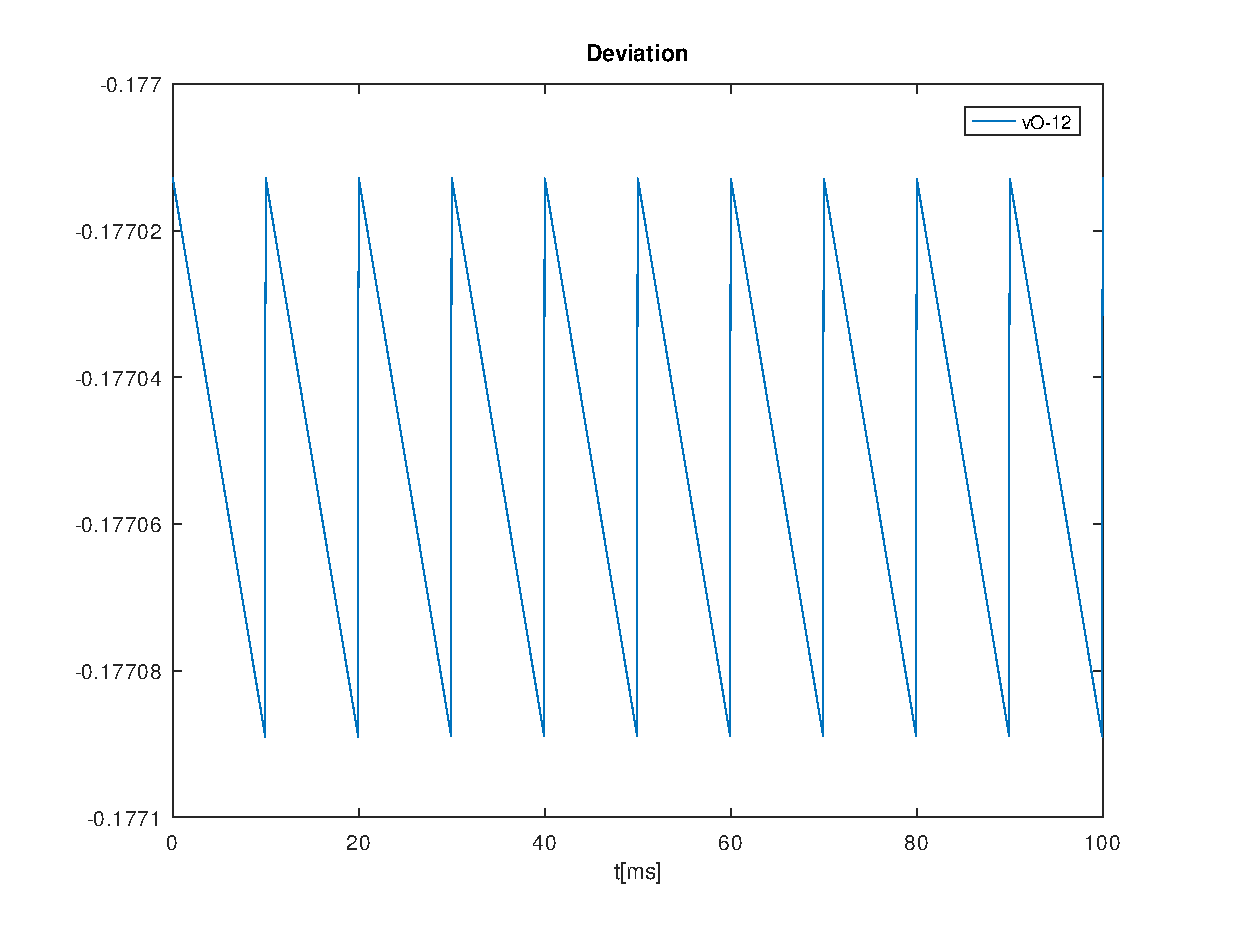
\includegraphics[width=0.8 \linewidth]{vdeviation.eps}
\caption{Deviation of $v_O$ from the 12V in funtion of time.}
\label{fig:env}
\end{figure}




